\chapter{Lectures}

\section{Lecture 6: 04.09.2025}

Now let's consider more complex BCs
\begin{align*}
    -\Delta \mathbf{u}                 & = \mathbf{f} \quad \text{in } \Omega   \\
    \mathbf{u}                         & = \mathbf{g} \quad \text{on } \Gamma_D \\
    \nabla \mathbf{u} \cdot \textbf{n} & = l \quad \text{on } \Gamma_N
\end{align*}
where $\Gamma_D \cup \Gamma_N = \partial \Omega$ and $\Gamma_D \cap \Gamma_N = \emptyset$.

We again test with an arbitrary function $\mathbf{v}$:
\begin{align*}
    \langle \mathbf{f}, \mathbf{v} \rangle & = \langle -\Delta \mathbf{u}, \mathbf{v} \rangle = \langle \nabla \mathbf{u}, \nabla \mathbf{v} \rangle + \int_{\partial \Omega} \nabla \mathbf{u} \cdot \textbf{n} \, \mathbf{v} \, ds
\end{align*}
As we have multiple BCs, on different subdomains we can consider them independently.
\begin{align*}
    \int_{\partial \Omega} \nabla \mathbf{u} \cdot \textbf{n} \, \mathbf{v} \, ds & = \int_{\Gamma_D} \nabla \mathbf{u} \cdot \textbf{n} \, \mathbf{v} \, ds + \int_{\Gamma_N} \nabla \mathbf{u} \cdot \textbf{n} \, \mathbf{v} \, ds = 0 + \int_{\Gamma_N} l \, \mathbf{v} \, ds
\end{align*}

\begin{itemize}
    \item \textbf{Neumann:} The natural BC becomes:
          \[
              \int_{\Gamma_N} \nabla \mathbf{u} \cdot \textbf{n} \, \mathbf{v} \, ds = \int_{\Gamma_N} l \, \mathbf{v} \, ds
          \]
          and remains in our formulation.
    \item \textbf{Dirichlet:} By specifying $\mathbf{u} \in \mathcal{H}^1_{\Gamma_D}(\Omega)$ where $\mathcal{H}^1_{\Gamma_D}(\Omega) = \{ \mathbf{v} \in \mathcal{H}^1(\Omega) : \mathbf{v}\vert_{\Gamma_D} = \mathbf{g} \}$ we obtain the weak form:
          \[
              \text{Find } \mathbf{u} \in \mathcal{H}^1_{\Gamma_D}(\Omega) \text{ s.t. } \langle \nabla \mathbf{u}, \nabla \mathbf{v} \rangle = \langle \mathbf{f}, \mathbf{v} \rangle + \int_{\Gamma_N} l \, \mathbf{v} \, ds \quad \forall \mathbf{v} \in \mathcal{H}^1_0(\Omega)
          \]
\end{itemize}

\textbf{Warning:} Trial and test spaces dont match! And $\mathcal{H}^1_{\Gamma_D}(\Omega) \nsubset \mathcal{H}^1(\Omega)$.
\textbf{Solution:} Lift the solution $\mathbf{u}$ so we solve a homogeneous problem.
Suppose we have operator $R_g \in \mathcal{H}^1(\Omega)$ s.t. $R_g\vert_{\Gamma_D} = \mathbf{g}$, then we set $\odot{\mathbf{u}} = \mathbf{u} - R_g$ and solve for $\odot{\mathbf{u}}$:
\[
    \text{Find } \odot{\mathbf{u}} \in \mathcal{H}^1_D(\Omega) \text{ s.t. } \langle \nabla \odot{\mathbf{u}}, \nabla \mathbf{v} \rangle = \langle \mathbf{f}, \mathbf{v} \rangle + \int_{\Gamma_N} l \, \mathbf{v} \, ds - \langle \nabla R_g, \nabla \mathbf{v} \rangle \quad \forall \mathbf{v} \in \mathcal{H}^1_D(\Omega)
\]
where
\[
    \mathcal{H}^1_D(\Omega) = \{ \mathbf{v} \in \mathcal{H}^1(\Omega) : \mathbf{v}\vert_{\Gamma_D} = 0 \}
\]
Thus the problem is \emph{symmetric} again!

\textit{Exercise:} More general elliptic problems:

Find the weak form for the PDE
\begin{align*}
    -\operatorname{div}{(\mu \nabla \mathbf{u})} + \sigma \mathbf{u} & = \mathbf{f} \quad \text{in } \Omega   \\
    \mathbf{u}                                                       & = \mathbf{g} \quad \text{on } \Gamma_D \\
    \mu \nabla \mathbf{u} \cdot \textbf{n}                           & = l \quad \text{on } \Gamma_N
\end{align*}

\subsection*{Functional analysis recap (also see Q2)}
A functional $F$ on $V$ is an operator mapping $F: V \to \mathbb{R}$.
The functional we have in mind is :
\[F = \langle \mathbf{f}, \mathbf{v} \rangle\]
A linear functional is said to be bounded if $\exists C > 0$ s.t.
\[|F(\mathbf{v})| \leq C \|\mathbf{v}\|_V \quad \forall \mathbf{v} \in V\]
If a functional is linear and bounded on some Banach space, then it is continuous.

\textit{Banach space: }
\begin{itemize}
    \item A vector space $V$ over $\mathbb{R}$ or $\mathbb{C}$
    \item Equipped with a norm $\|\cdot\|_V$
    \item Complete w.r.t. the metric induced by the norm
\end{itemize}

A bilinear form $a: V \times V \to \mathbb{R}$ is continuous if $\exists M > 0$ s.t.
\[|a(\mathbf{u}, \mathbf{v})| \leq M \|\mathbf{u}\|_V \|\mathbf{v}\|_V \quad \forall \mathbf{u}, \mathbf{v} \in V\]
and coercive if $\exists \alpha > 0$ s.t.
\[a(\mathbf{v}, \mathbf{v}) \geq \alpha \|\mathbf{v}\|_V^2 \quad \forall \mathbf{v} \in V\]

\begin{theorem}{Lax-Milgram}{}
    Let $V$ be a Hilbert space, $a(\cdot, \cdot): V \times V \to \mathbb{R}$ a continuous and coercive bilinear form, and $F: V \to \mathbb{R}$ a continuous linear functional. Then there exists a unique solution to the problem:
    \[
        \text{Find } \mathbf{u} \in V \text{ s.t. }
        a(\mathbf{u}, \mathbf{v}) = F(\mathbf{v}) \quad \forall \mathbf{v} \in V
    \]
    Moreover, $\|\mathbf{u}\|_V \leq \frac{1}{\alpha} \|F\|_{V'}$ where $\|F\|_{V'} = \sup_{\mathbf{v} \in V \setminus \{0\}} \frac{|F(\mathbf{v})|}{\|\mathbf{v}\|_V}$.
\end{theorem}
\begin{itemize}
    \item Based on \emph{Riesz representation theorem} and the \emph{Banach fixed point theorem}.
    \item To prove unique solutions exists we need to satisfy the conditions on the linear $F$ and bilinear form $a(\cdot, \cdot)$.
\end{itemize}

\begin{example}{}{}
    Consider seeking $u \in H^1_0([0, 1])$ s.t.

    \begin{align*}
        \int_0^1 u'(x) v'(x) \, dx & = \int_0^1 \sin(2\pi x) v(x) \, dx \quad \forall v \in H^1_0([0, 1]) \\
        a(u, v)                    & = \int_0^1 u'(x) v'(x) \, dx                                         \\
        F(v)                       & = \int_0^1 \sin(2\pi x) v(x) \, dx
    \end{align*}
    Clearly
    \begin{align*}
        |F(v)|        & \leq \|\sin(2\pi x)\|_{L^2} \|v\|_{L^2} \leq \|v\|_{L^2} \leq \|v\|_{H^1_0} \\
        \|v\|_{H^1}^2 & = \|v\|_{L^2}^2 + \|\nabla v\|_{L^2}^2 \geq \|v\|_{L^2}^2
    \end{align*}
    so $F$ is bounded and linear. Also
    \begin{align*}
        |a(u, v)| & = |\langle u, v \rangle_{H^1_0}| \leq \|u\|_{H^1_0} \|v\|_{H^1_0} \quad \text{(Cauchy-Schwarz)}
    \end{align*}
    thus continuous. For coercivity we must use the Poincaré inequality:
    \[\|v\|_{L^2} \leq C \|\nabla v\|_{L^2} \quad \forall v \in H^1_0(\Omega)\]
    so
    \begin{align*}
        a(v, v) & = \|\nabla v\|_{L^2}^2 \geq \frac{1}{C^2} \|v\|_{L^2}^2 \geq \frac{1}{C^2 + 1} \|v\|_{H^1_0}^2
    \end{align*}
    and we have coercivity.
    Thus by Lax-Milgram a unique solution exists.
\end{example}

\subsection*{Elliptic finite elements in 1D}
We have discussed the infinitely dimensional case, now we want to move into the finite dimensional case.

\begin{definition}{Ritz-Galerkin approximation}{}
    Let $a: \mathbb{V} \times \mathbb{V} \to \mathbb{R}$ be a bilinear form, and $\mathbb{V}_h \subset \mathbb{V}$ a finite dimensional subspace.
    Consider the weak form restricted to $\mathbb{V}_h$:
    \[\text{Find } \mathbf{u}_h \in \mathbb{V}_h \quad \text{s.t.} \quad a(\mathbf{u}_h, \mathbf{v}) = F(\mathbf{v}) \quad \forall \mathbf{v} \in \mathbb{V}_h\]
    This is called a Ritz-Galerkin approximation of the weak solution $\mathbf{u} \in \mathbb{V}$.
\end{definition}

\begin{example}{Polynomial subspace for the 1D problem}{}
    Consider a (naive) approx. of the form:
    \[
        \hat{u}(x) = a_0 + a_1 x + a_2 x^2 + a_3 x^3
    \]
    to our 1D problem:
    \begin{align*}
        -u''(x) & = f(x) \quad x \in (0, 1) \\
        u(0)    & = 0                       \\
        u'(1)   & = 0
    \end{align*}
    with the weak form:
    \[\text{Find } u \in H^1_0(0, 1) \quad \text{s.t.} \quad a(u, v) = F(v) \quad \forall v \in H^1_0(0, 1)\]
    where
    \begin{align*}
        a(u, v) & = \int_0^1 u'(x) v'(x) \, dx \\
        F(v)    & = \int_0^1 f(x) v(x) \, dx
    \end{align*}
    We observe that $\hat{u}(0) = a_0 = 0$ so we can rewrite:
    \[
        \hat{u}(x) = a_1 x + a_2 x^2 + a_3 x^3
    \]
    The monomials form a polynomial basis of a subspace of $\mathbb{V}_h \subset \mathbb{V}$ where we consider an approx. over a single element. The coefficients of $\hat{u}$ are determined by the constraints:
    \begin{align*}
        \langle \hat{u}', 1 \rangle    & = \langle f, x \rangle   \\
        \langle \hat{u}', 2x \rangle   & = \langle f, x^2 \rangle \\
        \langle \hat{u}', 3x^2 \rangle & = \langle f, x^3 \rangle
    \end{align*}
    This is because we want to satisfy the weak form for all $v \in \mathbb{V}_h$ and we have three basis functions.
    This gives us a linear system of equations for the coefficients $a_1, a_2, a_3$.
    \begin{align*}
        \begin{bmatrix}
            1 & 1           & 1           \\
            1 & \frac{4}{3} & \frac{3}{2} \\
            1 & \frac{3}{2} & \frac{9}{5}
        \end{bmatrix}
        \begin{bmatrix}
            a_1 \\
            a_2 \\
            a_3
        \end{bmatrix}
         & =
        \begin{bmatrix}
            \langle f, x \rangle   \\
            \langle f, x^2 \rangle \\
            \langle f, x^3 \rangle
        \end{bmatrix}
        = \begin{bmatrix}
              1                  \\
              -\frac{4}{\pi} + 2 \\
              \frac{\pi^2}{4} \left(-\frac{96}{\pi^4} + \frac{12}{\pi^2} \right)
          \end{bmatrix}
    \end{align*}
    which we can solve for:
    \[
        \hat{u}(x) \approx 1.6x - 0.16x^2 - 0.44x^3
    \]
    which remains close to the true solution
    \[
        u(x) = \sin(\frac{\pi x}{2}) \text{ over } [0, 1]
    \]
\end{example}

\textbf{Questions:}
\begin{itemize}
    \item Does a discrete solution always exist?
    \item Is it unique?
    \item How accurate is it?
\end{itemize}

\begin{theorem}{1D existence and uniqueness for $-u''(x) = f(x)$ with $u(0) = u'(1) = 0$}{}
    If $f \in L^2([0, 1])$ then $\exists! u_h$ to the Ritz-Galerkin approx. when $\mathbb{V}_h \subset \mathbb{V}$ is finite dimensional.
\end{theorem}
Since $\mathbb{V}_h$ is finite dimensional it has a finite dimensional basis:
\[\mathbb{V}_h = \text{span}\{\phi_1, \phi_2, \ldots, \phi_N\}\]
So, for any $u_h \in \mathbb{V}_h$ where:
\begin{align*}
    u_h(x)         & = \sum_{i=1}^n \alpha_i \phi_i(x) \\
    \symbf{\alpha} & = \{\alpha_i\}_{i=1}^n
\end{align*}
The Ritz-Galerkin approx. seeks $\symbf{\alpha}$ s.t.
\begin{align*}
    a(u_h, v)                                     & = F(v) \quad \forall v \in \mathbb{V}_h               \\
    a\left(\sum_{i=1}^n \alpha_i \phi_i, v\right) & = \langle f, \phi_j \rangle \quad j = 1, 2, \ldots, n
\end{align*}
Since any $v \in \mathbb{V}_h$ is also a linear combination of basis functions this is equivalent to seeking $\symbf{\alpha}$ s.t.
\begin{align*}
    a\left(\sum_{i=1}^n \alpha_i \phi_i, \phi_j\right) & = \langle f, \phi_j \rangle \quad j = 1, 2, \ldots, n
\end{align*}
where the rhs is finite as $f \in L^2([0, 1])$.

Through bilinearity:
\begin{align*}
    \sum_{i=1}^n \alpha_i a(\phi_i, \phi_j) & = \langle f, \phi_j \rangle, \quad j = 1, 2, \ldots, n
\end{align*}
Defining the matrix $A$ by $A_{ij} = a(\phi_i, \phi_j)$ and the vector $\mathbf{b}$ by $b_j = \langle f, \phi_j \rangle$, our approximation is equivalent to solving the linear system:
\[A \symbf{\alpha} = \mathbf{b}\]
Existence and uniqueness is equivalent to solving $A \symbf{\alpha} = \mathbf{b}$.
Assume $A$ is singular, i.e.
\[
    \exists \symbf{\beta} \neq 0 \text{ s.t. } A \symbf{\beta} = 0
\]
and
\[
    \symbf{\beta}^\top A \symbf{\beta} = 0
\]
We now define:
\[
    \tilde{v}(x) = \sum_{i=1}^n \beta_i \phi_i(x) \in \mathbb{V}_h
\]
We see that:
\begin{align*}
    \symbf{\beta}^\top A \symbf{\beta} & = \sum_{i=1}^n \sum_{j=1}^n \beta_i a(\phi_i, \phi_j) \beta_j \\
                                       & = a(\sum_{i=1}^n \beta_i \phi_i, \sum_{j=1}^n \beta_j \phi_j) \\
                                       & = a(\tilde{v}, \tilde{v})= \int_0^1 \tilde{v}'(x)^2 \, dx = 0
\end{align*}
Now, if:
\begin{align*}
    \symbf{\beta}^\top A \symbf{\beta} = 0 \implies \tilde{v}'(x) = 0 \, \forall x, implies \tilde{v}(x) = C \\
\end{align*}
As $\tilde{v} \in \mathbb{V}_h \subset \mathbb{V} = H^1_0([0, 1])$ it must satisfy the BC $\tilde{v}(0) = 0$ so $C = 0$ and $\symbf{\beta} = 0$ which is a contradiction.
As $A$ must be non-singular, $A \symbf{\alpha} = \mathbf{b}$ has a unique solution $\symbf{\alpha}$ and thus a unique solution.

\section{Lecture 7: 10.09.2025}
\begin{lemma}{Galerkin Orthogonality}{}
    Let $u \in V$ be the solution to the weak form and $u_h \in V_h \subset V$ the Ritz-Galerkin approximation.

    \[
        a(u - u_h, v) = 0 \quad \forall v \in V_h
    \]
\end{lemma}
Recall the weak form:
\[
    a(u, v) = F(v) \quad \forall v \in V
\]
and the Ritz-Galerkin approx.:
\[
    a(u_h, v) = F(v) \quad \forall v \in V_h
\]
As $V_h \subset V$ through restricting the weak form and:
\[
    a(u - u_h, v) = \langle f, v \rangle - \langle f, v \rangle = 0 \quad \forall v \in V_h
\]

\subsection{Cea's Lemma Vol. 1 (Optimality of Ritz-Galerkin approximation)}
\begin{lemma}{Cea's Lemma}{ceas-lemma}
    If $u \in V$ solves the weak form and $u_h \in V_h$ the Ritz-Galerkin approximation, then:
    \[
        \|u - u_h\|_V = \min_{v \in V_h} \|u - v\|_V
    \]
\end{lemma}

Recall that:
\[
    \|u - u_h\|_V^2 = a(u - u_h, u - u_h)
\]
For any $v \in V_h$ we have:
\begin{align*}
    a(u - u_h, u - u_h) & = a(u - u_h, u - v) + a(u - u_h, v - u_h)
\end{align*}

Noting that $v - u_h \in V_h$ we use Galerkin orthogonality to eliminate the second term:
\begin{align*}
    \|u - u_h\|_V^2 & = a(u - u_h, u - v) \quad \forall v \in V_h
\end{align*}
As $a(\cdot, \cdot)$ is an inner product (continuous and coercive) we can use the Cauchy-Schwarz inequality:
\begin{align*}
    \|u - u_h\|_V^2 & \leq \|u - u_h\|_V \|u - v\|_V \quad \forall v \in V_h
\end{align*}
as the statement holds for all $v \in V_h$ it also holds for the minimiser:
\[\|u - u_h\|_V^2 \leq \|u - u_h\|_V \min_{v \in V_h} \|u - v\|_V \qed\]

Before proving error estimates in 1D we need some assumptions and results:
\begin{itemize}
    \item \textbf{Approximation assumption:} Given $V_h \subset V$, assume for $V_h$ there $\exists \varepsilon > 0$ s.t. $\forall u \in C^2([0, 1]) \cap V$ where:
          \[
              \min_{v \in V_h} \|u - v\|_V \leq \varepsilon \|u''\|_{L^2}
          \]
    \item \textbf{Theorem: Aubin-Nitsche duality argument:}
          Let $f \in L^2([0, 1])$, $u \in V$ solves the weak form and $u_h \in V$ the Ritz-Galerkin approx. If the approx. assumption holds then:
          \[\|u - u_h\|_{L^2} \leq \varepsilon \|u - u_h\|_V\]
          \emph{Proof:}
          Let $w \in C^2([0, 1]) \cap V$ solve the dual problem:
          \begin{align*}
              -w''  & = u - u_h, \quad x \in (0, 1) \\
              w(0)  & = 0                           \\
              w'(1) & = 0
          \end{align*}
          Then $w$ solves the weak form:
          \[a(w, v) = \langle u - u_h, v \rangle \quad \forall v \in V\]
          Since $u - u_h \in V$ we have:
          \begin{align*}
              \|u - u_h\|_{L^2}^2 & = \langle u - u_h, u - u_h \rangle = a(w, u - u_h)                                       \\
                                  & = a(w, u - u_h) - a(u - u_h, v) \quad \forall v \in V_h \text{ (Galerkin orthogonality)}
          \end{align*}
          Through Galerkin orthogonality. Through Cauchy-Schwarz (CS):
          \[
              \|u - u_h\|_{L^2}^2 \leq \|u - u_h\|_V \|w - v\|_V \quad \forall v \in V_h
          \]
          Choosing $v$ to be the minimiser we can use the approx. assumption:
          \[
              \|u - u_h\|_{L^2}^2 \leq \varepsilon \|u - u_h\|_V \|w''\|_{L^2} = \varepsilon \|u - u_h\|_V \|u - u_h\|_{L^2}
          \]
          by construction of the dual problem, thus:
          \[
              \|u - u_h\|_{L^2} \leq \varepsilon \|u - u_h\|_V \qed
          \]
\end{itemize}

\begin{corollary}{}{}
    Let the assumptions of \emph{Aubin-Nitsche} hold. If $f \in C^0([0, 1])$ and $u \in C^2([0, 1])$, then:
    \[
        \|u - u_h\|_{L^2} \leq \varepsilon \|u - u_h\|_V \leq \varepsilon^2 \|f\|_{L^2}
    \]
\end{corollary}
From \ref{lem:ceas-lemma} we have:
\[\|u - u_h\|_V = \min_{v \in V_h} \|u - v\|_V\]
and the approx. assumption:
\[\min_{v \in V_h} \|u - v\|_V \leq \varepsilon \|u''\|_{L^2}\]
we see that:
\[\varepsilon \|u - u_h\|_V \leq \varepsilon \min_{v \in V_h} \|u - v\|_V \leq \varepsilon^2 \|u''\|_{L^2}.\]
Since $u \in C^2([0, 1])$ it is a strong solution of the PDE and $\|u''\|_{L^2} = \|f\|_{L^2}$ allowing us to conclude:
\[\|u - u_h\|_{L^2} \leq \varepsilon \|u - u_h\|_V \leq \varepsilon^2 \|f\|_{L^2} \qed\]

\subsection{Meshes}
\begin{definition}{Mesh}{mesh}
    A mesh on $[0, 1]$ is given by a set of nodes satisfying:
    \[0 = x_0 < x_1 < x_2 < \ldots < x_n= 1\]
    which divide $[0, 1]$ into $n$ elements:
    \[I_i = [x_i, x_{i+1}], \quad i = 0, 1, \ldots, n-1\]
    The mesh spacing is defined by $h_i = x_{i+1} - x_i$.
\end{definition}

\begin{definition}{Finite Element Space}{fe-space}
    For $k \geq 1$ we define:
    \begin{align*}
        V_h^k & = \{v \in C^0([0, 1]) : v(x) \text{ is polynomial of degree }\leq k \text{ on each element } I_i \text{ and } v(0) = 0\} \\
              & = \{v \in C^0([0, 1]) : v(x)\vert_{I_i} \in \mathbb{P}_k, \, i = 0, 1, \ldots, n-1, \, v(0) = 0\}
    \end{align*}
\end{definition}

\section{Lecture 8: 11.09.2025}

Recall if $k=1$ we may use nodal basis functions:

\[
    \phi_i(x)
    = \begin{cases}
        \frac{x - x_{i-1}}{x_i - x_{i-1}}, & x \in [x_{i-1}, x_i] =  I_{i-1} \\
        \frac{x_{i+1} - x}{x_{i+1} - x_i}, & x \in [x_i, x_{i+1}] = I_i      \\
        0,                                 & \text{otherwise}
    \end{cases}
    \quad i = 1, 2, \ldots, n-1
\]

With the last basis function given by:
\[
    \phi_n(x)
    = \begin{cases}
        \frac{x - x_{n-1}}{x_n - x_{n-1}}, & x \in [x_{n-1}, x_n] =  I_{n-1} \\
        0,                                 & \text{otherwise}
    \end{cases}
\]

Now we have defined $V_h$, we can study the error.

\begin{theorem}{}{}
    Let $h = \max_i h_i$, $w \in C^2([0, 1]) \cap V_h^1$ and the interpolant $I w$. Then:
    \[
        \|w - Iw\|_V \leq \frac{h}{\sqrt{2}} \|w''\|_{L^2}
    \]

\end{theorem}
\begin{proof}
    We begin by restricting to an arbitrary element $I_i$ noting:
    \[
        \|w - I w\|_V^2 = \sum_{i=0}^{n-1} \int_{I_i} (\left[w(x) - I w(x)\right]')^2 \, dx
    \]
    and:
    \[
        \|w''\|_{L^2}^2 = \sum_{i=0}^{n-1} \int_{I_i} \left[w''\right]^2 \, dx = \sum_{i=0}^{n-1} \int_{I_i} \left[w'' - (I w)''\right]^2 \, dx
    \]
    as $(I w)'' = 0$ on $I_i$.

    Let/write $e(x) = w(x) - I w(x)$, then we want to show:
    \[
        \int_{I_i} (e'(x))^2 \, dx \leq \frac{(x_{i+1} - x_i)^2}{2} \int_{I_i} (e''(x))^2 \, dx
    \]
    To simplify we remap our element $I_i \mapsto [0, 1]$.

    Let $x = x_i + s(x_{i+1} - x_i)$ for $s \in (0, 1)$ and define $\tilde{e}(s) = e(x_i + s(x_{i+1} - x_i))$.
    Then:
    \begin{align*}
        \frac{d\tilde{e}}{ds}     & = h_i e'(x_i + s (x_{i+1} - x_i) )    \\
        \frac{d^2\tilde{e}}{ds^2} & = h_i^2 e''(x_i + s (x_{i+1} - x_i) )
    \end{align*}

    Allowing us to express what we want to show as:
    \[
        \int_0^1 \left(\frac{d\tilde{e}}{ds}\right)^2 \, ds \leq \frac{1}{2} \int_0^1 \left(\frac{d^2\tilde{e}}{ds^2}\right)^2 \, ds
    \]
    Note: we have defined $\tilde{e}(s)$ so it matches $e(x)$ at the nodes:
    \[
        \tilde{e}(x_i) = e(x_{i + 1}) = 0 \implies \tilde{e}(0) = \tilde{e}(1) = 0
    \]
    As $w$ and $I w$ are continuous and differentiable, so is $\tilde{e}$.

    Using \emph{Rolle's theorem}:

    \[
        \exists \xi \in (0, 1) \text{ s.t. } \tilde{e}'(\xi) = \int_{\xi}^s \tilde{e}''(t) \, dt \quad \forall s \in [0, 1]
    \]
    Using Cauchy-Schwarz (CS):
    \begin{align*}
        |\tilde{e}'(s)| & = \left|\int_{\xi}^s \tilde{e}''(s) \, ds\right| \leq \left(\int_{\xi}^s \, ds\right)^{1/2} \left(\int_{\xi}^s \left[\tilde{e}''(s)\right]^2 \, ds\right)^{1/2} \\
                        & \leq \left|s - \xi\right|^{1/2} \left(\int_0^s \left[\tilde{e}''(s)\right]^2 \, ds\right)^{1/2}
    \end{align*}
    Squaring and integrating over $s \in [0, 1]$:
    \begin{align*}
        \int_0^1 \left[\tilde{e}'(s)\right]^2 \, ds & \leq \left(\int_0^1 |s - \xi| \, ds\right) \left(\int_0^1 \left[\tilde{e}''(s)\right]^2 \, ds\right)
    \end{align*}
    Noting that:
    \[
        \int_0^1 |s - \xi| \, ds = \xi^2 - \xi + \frac{1}{2} \leq \frac{1}{2} \quad \forall \xi \in (0, 1)
    \]
    We obtain:
    \[
        \int_0^1 \left[\tilde{e}'(s)\right]^2 \, ds \leq \frac{1}{2} \int_0^1 \left[\tilde{e}''(s)\right]^2 \, ds
    \]
    Allowing us to conclude.\qed
\end{proof}

\begin{corollary}{$\mathbb{P}_1$ error estimate for the Ritz-Galerkin approx. $u_h \in V_h^1$}{}
    Let $f \in C^0([0, 1])$ and $u \in C^2([0, 1]) \cap V$. Let $u_h$ be the Ritz-Galerkin approx. of $u \in V$ over $V_h^1$ i.e.
    \[
        a(u_h, v) = \langle f, v \rangle \quad \forall v \in V_h^1
    \]
    Then:
    \[
        \|u - u_h\|_{L^2} \leq \frac{h}{\sqrt{2}} \|u - u_h\|_V \leq \frac{h^2}{2} \|f\|_{L^2}
    \]
\end{corollary}

\begin{corollary}{Approximation property for $V_h^k$}{}
    Approximation property for $V_h^k$: Let $h = \max_i h_i$, $w \in C^2([0, 1]) \cap V$, then:
    \[
        \min_{v \in V_h^k} \|w - v\|_V \leq \frac{h}{\sqrt{2}} \|w''\|_{L^2}
    \]
\end{corollary}
This follows immediately from $V_h^1 \subset V_h^k$. This is not an optimal error bound and in practice we expect to gain one order (power of $h$) per polynomial degree. Higher order error bounds will require higher regularity on the weak solution $u$.\footnote{Password for lecture notes: FiniteElement314159}

\subsection{Existence and uniqueness}

\paragraph{Functional analysis recap:} Recall the function space:
\[
    C^m(\Omega) = \{f \in C^0(\Omega) : D^{\mathbf{k}} f \in C^0(\Omega) \quad \forall |\mathbf{k}| \leq m\}
\]
where:
\begin{align*}
    |\mathbf{k}|   & = k_1 + k_2 + \ldots + k_d                                                                        \\
    D^{\mathbf{k}} & = \frac{\partial^{|\mathbf{k}|}}{\partial x_1^{k_1} \partial x_2^{k_2} \ldots \partial x_d^{k_d}}
\end{align*}
Now define:
\begin{align*}
    C^\infty(\Omega) & = \{ f \in C^0(\Omega) : D^{\mathbf{k}} f \in C^0(\Omega) \quad \forall \mathbf{k} \} \tag{infinitly smooth} \\
    C_0^m(\Omega)    & = \{ f \in C^m(\Omega) : \text{supp}(f) \subset \subset \Omega \} \tag{compact support}
\end{align*}
Where the support of $f(x)$ is the closure of the set of points where $f(x) \neq 0$, and $f(x)$ is compactly supported when the support of $f(x)$ is a compact set in $\mathbb{R}^n$.

\begin{example}{}{}
    Let $\Omega = \mathbb{R}$, then:
    \begin{align*}
        f(x) & =
        \begin{cases}
            4(x - x^2), & x \in (0, 1)     \\
            0,          & \text{otherwise}
        \end{cases}
    \end{align*}
    is compact in $\mathbb{R}$, as $4(x - x^2)$ takes the values $0$ at $x = 0, 1$. The function is $C_0^0(\Omega)$, but as
    \[
        \frac{d}{dx}\left(4(x - x^2)\right)\vert_{x = 1} = -4 \neq 0
    \]
    it fails to be $C_0^1(\Omega)$.
\end{example}

To design $g(x) \in C_0^k(\Omega)$ for $k < \infty$ we can choose $g(x) = f(x)^{k+1}$.
Given a normed vector space $V$, a sequence of functions $\{f_i\}_{i=1}^\infty \subset V$ or $f_i \in V$ is said to converge to a limit if:
\[
    \lim_{i \to \infty} \|f_i - f\|_V = 0
\]

The sequence $\{f_i\}_{i=1}^\infty$ is a Cauchy sequence if:
\[
    \forall \varepsilon > 0 \, \exists N \in \mathbb{N} \text{ s.t. } \|f_i - f_j\|_V < \varepsilon \quad \forall i, j > N
\]

\begin{definition}{Banach space}{banach-space}
    Is a complete normed vector space for which every Cauchy sequence $\{f_i\}_{i=1}^\infty\}$ has a limit $f \in V$.
\end{definition}

\begin{definition}{$L^p$ spaces}{lp-spaces}
    For $1 \leq p < \infty$ we define:
    \begin{align*}
        L^p(\Omega) & = \{u : u \text{ is real and measurable }, \int |u(x)|^p \, dx < \infty\} \\
        \|u\|_p     & = \left(\int_\Omega |u(x)|^p \, dx\right)^{\frac{1}{p}} \tag{norm}
    \end{align*}
    For $p = \infty$ we define:
    \begin{align*}
        L^\infty(\Omega) & = \{u : |u(x)| < \infty \text{ a.e. in } \Omega\}   \\
        \|u\|_\infty     & = \inf\{C : |u(x)| \leq C \text{ a.e. in } \Omega\}
    \end{align*}
\end{definition}

\paragraph{Inequalities in $L^p$ spaces:}
\begin{itemize}
    \item \textbf{Hölder's inequality:} For $1 \leq p, q \leq \infty$ with $\frac{1}{p} + \frac{1}{q} = 1$ we have:
          \[
              \|uv\|_1 \leq \|u\|_p \|v\|_q
          \]
    \item \textbf{Minkowski's inequality:} For $1 \leq \leq \infty$ we have:
          \[
              \|u + v\|_p \leq \|u\|_p + \|v\|_p
          \]
\end{itemize}

\paragraph{Hilbert spaces} is an inner product space which is complete w.r.t. the norm induced by the inner product $\langle \cdot, \cdot \rangle^{\frac12} = \|\cdot\|$.

\begin{theorem}{Hilbert projection}{hilbert-projection}
    Let $\mathcal{M} \subset V$ be a closed subspace of a Hilbert space $V$. Then:
    \[
        \forall u \in V \, \exists! v \in \mathcal{M} \text{ and } w \in \mathcal{M}^\perp \text{ s.t. } u = v + w
    \]
    where
    \begin{align*}
        \mathcal{M}^\perp & = \{w \in V : \langle v, w \rangle_V = 0 \quad \forall v \in \mathcal{M}\} \\
        V                 & = \mathcal{M} \oplus \mathcal{M}^\perp
    \end{align*}
\end{theorem}

We define the space of locally integrable functions:
\[
    L_{\text{loc}}^1(\Omega) = \{u(x) : \int_{\Omega} |u(x) \phi(x)| \, dx < \infty \quad \forall \phi \in C_0^\infty(\Omega)\}
\]
Note that:
\[
    L^1(\Omega) \subset L_{\text{loc}}^1(\Omega)
\]
as it enforces compact support for solutions which may blow up at the boundary (e.g. $u(x) = \frac1x$ on $\Omega = [0, 1]$).

\begin{definition}{Weak derivative}{weak-derivative}
    $v \in L_{\text{loc}}^1(\Omega)$ is the weak partial derivative of $u \in L_{\text{loc}}^1(\Omega)$ in the $k$-th component if:
    \[
        \int_\Omega v \phi \, dx = -\int_\Omega u \frac{\partial \phi}{\partial x_k} \, dx \quad \forall \phi \in C_0^\infty(\Omega)
    \]
\end{definition}

For higher order derivative let $\symbf{\alpha}$ be a multi-index:
\[\symbf{\alpha} = (\alpha_1, \alpha_2, \ldots, \alpha_d) \quad \alpha_i \in \mathbb{N}_0\]
then the $|\symbf{\alpha}|$ order partial derivative  $v$ is:
\[
    \int_\Omega v \phi \, dx = (-1)^{|\symbf{\alpha}|} \int_\Omega u \frac{\partial^{|\symbf{\alpha}|} \phi}{\partial x_1^{\alpha_1} \partial x_2^{\alpha_2} \ldots \partial x_d^{\alpha_d}} \, dx \quad \forall \phi \in C_0^\infty(\Omega)
\]
We write this weak derivative as $v = D^{\symbf{\alpha}} u$.

\section{Lecture 9: 17.09.2025}

\begin{example}{Weak derivatives}{}
    Consider the function:
    \[
        f(x) =
        \begin{cases}
            2x,     & 0 \leq x \leq \frac{1}{2} \\
            2 - 2x, & \frac{1}{2} < x \leq 1
        \end{cases}
    \]
    This function isnt differentiable at $x = \frac12$, but weakly differentiable:
    \[
        D_{\mathrm{w}} f(x) =
        \begin{cases}
            2,      & 0 \leq x < \frac{1}{2} \\
            \alpha, & x = \frac{1}{2}        \\
            -2,     & \frac{1}{2} < x \leq 1
        \end{cases}
    \]
    Note that at $x = \frac12$ the pointwise value is \emph{immaterial} (meaning arbitrary) due to the integral in the definition of weak derivatives \autoref{def:weak-derivative}.
\end{example}

\subsection{Sobolev spaces}
\begin{definition}{Sobolev space}{lec:sobolev-space}
    Let $\Omega \subset \mathbb{R}^n$, $k \in \mathbb{N}_0$ and $1 \leq p < \infty$. The $(k, p)$-Sobolev space is defined as:
    \[
        W^{k, p}(\Omega) = \{u: \Omega \to \mathbb{R} \mid \|u\|_{k,p} < \infty\}
    \]
    where:
    \[
        \|u\|_{k,p}^p  = \sum_{|\symbf{\alpha}| \leq k} \|D_{\mathrm{w}}^{\symbf{\alpha}} u\|_{L^p}^p = \sum_{|\symbf{\alpha}| \leq k} \int_\Omega |D_{\mathrm{w}}^{\symbf{\alpha}} u|^p \, dx
    \]
\end{definition}

For $W^{0, 2}(\Omega) = L^2(\Omega)$. Typically one chooses $p = 2$, so we introduce the following notation $L^2$-Sobolev spaces.
\begin{definition}{$L^2$-Sobolev space}{}
    Let $\Omega \subset \mathbb{R}^n$, $k \in \mathbb{Z}^+$, then:
    \[
        H^k(\Omega) = W^{k, 2}(\Omega)
    \]
    which is a \emph{Hilbert space}.
\end{definition}

Consider the (new) elliptic Model Problem:

\begin{align*}
    -\nabla \cdot \nabla u(x) + u(x) & = f(x), \quad x \in \Omega \subset \mathbb{R}^n, \, f \in L^2(\Omega) \\
    u(x)                             & = 0, \quad x \in \partial \Omega
\end{align*}

The weak formulation is given by seeking $u \in V = H_0^1(\Omega)$ s.t.

\[
    \int_\Omega \nabla u \cdot \nabla v \, dx + \int_\Omega u v \, dx = \int_\Omega f v \, dx \quad \forall v \in V
\]

Equivalently we have:
\begin{align*}
    a(u, v) & = \int_\Omega \nabla u \cdot \nabla v \, dx + \int_\Omega u v \, dx \\
    g(v)    & = \int_\Omega f v \, dx
\end{align*}

\subsection{Existence and uniqueness of weak solutions}
To show existence and uniqueness we need to show that the bilinear form $a(\cdot, \cdot)$ is \emph{non-degenerate (coercive)}.

\begin{definition}{Bounded linear functional}{bounded-linear-functional}
    A linear functional $g: V \to \mathbb{R}$ is bounded if $\exists C > 0$ s.t.
    \[
        |g(v)| \leq C \|v\|_V \quad \forall v \in V.
    \]
\end{definition}

\subsection{Dual space}
Let $V$ be a Hilbert space with norm $\|\cdot\|_V$. The dual space $V^\star$ is the space of bounded linear functionals on $V$:
\[
    V^\star := \{g: V \to \mathbb{R} : g \text{ is a bounded linear functional}\}
\]
with the operator norm defined by:
\[
    \|g\|_{V^\star} := \sup_{\substack{u \in V \\ u \neq 0}} \frac{|g(u)|}{\|u\|_V}
\]

As $f \in L^2$ for (MP) $g(v) = \int_\Omega f v \, dx$.
This assumption can be relaxed as for $g(v)$.
\[
    |g(v)| = \left|\int_\Omega f(x) v \, dx\right| \quad \forall v \in H_0^1(\Omega)
\]
which can be bounded even if $f \notin L^2(\Omega)$.
Formally we introduce the (negative) Sobolev space $w \in H^{-1}(\Omega)$:\footnote{The negative Sobolev space is the dual space of $H_0^1(\Omega)$, i.e. $H^{-1}(\Omega) = (H_0^1(\Omega))^\star$, similarly $\|v\|_1 = \|v\|_{H^1}$ and $\langle f, v \rangle_0 = \langle f, v \rangle_{L^2}$.}
\[
    \|w\|_{-1} = \sup_{v \in H^1(\Omega)} \frac{|\langle w, v \rangle_0|}{\|v\|_{1}} < \infty
\]

\subsection{Riesz representation theorem}
\begin{theorem}{Riesz representation theorem}{riesz-representation-theorem}
    Let $V$ be a Hilbert space and $g \in V^\star$. Then $\exists! u \in V$ s.t.
    \[
        g(v) = \langle u, v \rangle_V \quad \forall v \in V.
    \]
\end{theorem}
\begin{proof}
    Consider $g \in V^\star$ and denote the kernel of $g$ by:
    \[
        \ker(g) = \{v \in V : g(v) = 0\}
    \]
    Denote $\mathcal{K} := \ker(g)$ which is a closed linear subspace. Let's split our argument into two cases:
    \begin{enumerate}
        \item If $\mathcal{K} = V$. Here for each $v \in V, g(v) = 0 \implies u = 0$.
        \item If $\mathcal{K} \neq V$. Consider $w \in \mathcal{K}^\perp$ where $w \neq 0$. Now let $y = g(w) \neq 0$. We observe that:
              \[
                  g(\frac{v}{y} w)  = \frac{g(v)}{y} g(w) = g(v) \quad \forall v \in V
              \]
              Through the linearity of $g(\cdot)$. Consequently:
              \begin{align*}
                  g(v - \frac{g(v)w}{y}) & = g(v) - g(v) = 0                                                           \\
                                         & \implies v - \frac{g(v)w}{y} \in \mathcal{K}                                \\
                                         & \implies \langle v - \frac{g(v)w}{y}, w \rangle_V = 0 \quad \forall v \in V
              \end{align*}
              as $w \in \mathcal{K}^\perp$ by Hilbert projection theorem, so we have:
              \[\langle \frac{g(v)}{y} w, w \rangle_V = \langle v, w \rangle_V \quad \forall v \in V\]
              leading to:
              \[
                  g(v) = \frac{\langle v, w \rangle_V}{\langle w, w \rangle_V} y = \langle v, u \rangle_V
              \]
              Through defining $u$ as:
              \[
                  u = \frac{w y}{\langle w, w \rangle_V}= \frac{w g(w)}{\langle w, w \rangle_V}
              \]
              Now we have found $u$. We must show that its unique.

              Suppose $\exists \hat{u} \in V$ s.t. $g(v) = \langle \hat{u}, v \rangle_V$ for all $v \in V$. Then:
              \[
                  g(v) = \langle u, v \rangle = \langle \hat{u}, v \rangle \quad \forall v \in V,
              \]
              showing that:
              \[
                  \langle u - \hat{u}, v \rangle_V = 0 \quad \forall v \in V.
              \]
              If $v \in u - \hat{u}$ then:
              \[
                  \langle u - \hat{u}, u - \hat{u} \rangle = 0 \implies u - \hat{u} = 0 \implies u = \hat{u}.
              \]
              Thus $u$ is unique.\qed
    \end{enumerate}
\end{proof}

\begin{corollary}{}{}
    For (MP) the bilinear form is the $H^1$ inner product:
    \[
        a(u, v) = \langle \nabla u, \nabla v \rangle + \langle u, v \rangle_{L^2} \quad \forall u, v \in H_0^1(\Omega),
    \]
    so our weak formulation is:
    \[
        g(v) = \langle u, v \rangle_{H^1} \quad \forall v \in H_0^1(\Omega).
    \]
    Through seeking $u \in H_0^1(\Omega)$ we satisfy the conditions of the Riesz representation theorem \ref{thm:riesz-representation-theorem} and so there exists a unique weak solution to (MP).
\end{corollary}

In general, not all weak forms are expressible with inner products on Hilbert spaces.

Consider:
\begin{align*}
    -\nabla \cdot \nabla u(x) & = f(x), \quad x \in \Omega \subset \mathbb{R}^n
    u(x)                      & = 0, \quad x \in \partial \Omega \text{ with } f \in L^2(\Omega)
\end{align*}
The weak form is given by seeking $u \in V$ s.t.
\begin{align*}
    a(u, v) & = \int_\Omega \nabla u \cdot \nabla v \, dx \\
    g(v)    & = \int_\Omega f v \, dx                     \\
    a(u, v) & = g(v) \quad \forall v \in V \tag{MP2}
\end{align*}

\subsection{V-ellipticity}

Given a Hilbert space $V$ consider a bilinear form $a: V \times V \to \mathbb{R}$. Then:
\begin{itemize}
    \item $a(\cdot, \cdot)$ is \textbf{coercive} if $\exists C_0 > 0$ s.t.
          \[
              C_0 \|u\|_V^2 \leq a(u, u) \quad \forall u \in V
          \]
    \item $a(\cdot, \cdot)$ is \textbf{continuous} if $\exists C_1 > 0$ s.t.
          \[
              |a(u, v)| \leq C_1 \|u\|_V \|v\|_V \quad \forall u, v \in V
          \]
    \item[$\implies$] if $a(\cdot, \cdot)$ is \textbf{coercive} and \textbf{continuous} on $V$ then $a(\cdot, \cdot)$ is called \textbf{$V$-elliptic}.
\end{itemize}

\subsection{Lax-Milgram (symmetric case)}
\begin{theorem}{Lax-Milgram (symmetric case)}{lax-milgram-symmetric}
    Let $V$ be a Hilbert space with inner product $\langle \cdot, \cdot \rangle_V$.
    Assume $a(\cdot, \cdot)$ is \textbf{symmetric} (i.e. $a(u, v) = a(v, u) \forall v,u \in V$) and \textbf{$V$-elliptic}, and that $g$ is a BLF (Bounded Linear Functional) on $V$.
    Then $\exists! u \in V$ s.t.
    \[
        a(u, v) = g(v) \quad \forall v \in V
    \]

\end{theorem}
\begin{proof}
    \begin{enumerate}
        \item $a(u, v) = a(v, u)$ by symmetry.
        \item $a(cu + w, v) = c a(u, v) + a(w, v)$ by bilinearity.
        \item $a(u, u) \geq C_0 \|u\|_V^2$ by coercivity.
        \item if $u = 0$ (a.e.), then $0 \leq a(u, u) \leq C_1 \|u\|_V^2 = 0$ and $a(u, u) = 0$ by \textbf{continuity}.
        \item if $a(u, u) = 0$ then $0 \leq C_1 \|u\|_V^2 \leq a(u, u) = 0 \implies u = 0$ (a.e.) by \textbf{coercivity}.
    \end{enumerate}
    Together these show $a(\cdot, \cdot)$ defines an inner prioduct on $V$ and we can conclude by the Riesz representation theorem \ref{thm:riesz-representation-theorem}.\qed
\end{proof}

\section{Lecture 10: 18.09.2025}
Note that if $a(\cdot, \cdot)$ is symmetric and $V$-elliptic it's norm is equivalent to the $V$-norm as:
\[
    c_0 \|u\|_V^2 \leq a(u, u) \leq C_1 \|u\|_V^2 \quad \forall u \in V
\]

\begin{theorem}{Lax-Milgram}{lax-milgram}
    Let $V$ be a Hilbert space, $a(\cdot, \cdot)$ be $V$-elliptic and $g(\cdot)$ be a BLF on $V$. Then $\exists! u \in V$ s.t.
    \[
        a(u, v) = g(v) \quad \forall v \in V
    \]
\end{theorem}
\begin{proof}
    For $u \in V$ note that $a_u(v) := a(u, v)$ is a BLF due to the continuity:
    \[
        |a_u(v)| = |a(u, v)| \leq C_1 \|u\|_V \|v\|_V \quad \forall v \in V
    \]
    So by the RRT $\exists! t_u \in V$ s.t.
    \[
        a_u(v) = \langle v, t_u \rangle_V \quad \forall v \in V
    \]
    Note that $a_u(v) = \langle v, t_u \rangle_V$ defines a mapping $T: V \to V$.

    For a given $u$, $t_u = T u$ is defined by RRT.

    Now we show that $T$ is linear and bounded on $V$:
    \begin{itemize}
        \item $T$ \textbf{is linear}: Consider $\alpha u + w \in V$ and $\alpha \in \mathbb{R}$, then for all $v \in V$:
              \begin{align*}
                  \langle v, T(\alpha u + w) \rangle_V & = a_{\alpha u + w}(v) = a(\alpha u + w, v) = \alpha a(u, v) + a(w, v)                 \\
                                                       & = \alpha a_u(v) + a_w(v) = \alpha \langle v, T u \rangle_V + \langle v, T w \rangle_V \\
                                                       & = \langle v, \alpha T u + T w \rangle_V
              \end{align*}
              So by the definiton of inner products $T(\alpha u + w) = \\alpha T u + T w$.
        \item $T$ \textbf{is bounded}: For $u \in V$ we have:
              \[
                  \|T u\|_V^2  = \langle T u, T u \rangle_V = a_u(T u) \leq C_1 \|T u\|_V \|u\|_V
              \]
              by continuity and:
              \[
                  \|T u\|_V \leq C_1 \|u\|_V \quad \forall u \in V \quad \implies \|T\| \leq C_1 < \infty
              \]
              Thus $T$ is bounded.
        \item $\range(T)$ \textbf{is closed}: Let $z_n = T u_n$ be a sequence in $\range(T)$, then:
              \[
                  a(u_n, v) = \langle v, T u_n \rangle_V = \langle v, z_n \rangle_V \quad \forall v \in V
              \]
              by choosing $v = u_n - u_m$ we have:
              \[
                  a(u_n - u_m, v)  = \langle v, z_n - z_m \rangle_V \quad \forall v \in V, \text{ and } C_0 \|u_n - u_m\|_V \leq \|z_n - z_m\|_V
              \]
              \textbf{If:} $z_n \to z \in V$ the sequence $u_n$ must be Cauchy. Since $V$ is a Hilbert space, $u_n$ must converge to some $u \in V$.
              By continuity $a(u_n, v) \to a(u, v)$. Note we have that:
              \[
                  |\langle T u_n - z, v \rangle_V| \to 0
              \]
              so $\langle v, T u_n \rangle_V \to \langle v, z \rangle_V$. Since $a(u_n, v) = \langle v, T u_n \rangle_V$ we see that $z = T u$. Thus since $z_n \to z \in \range(T)$, $\range(T)$ is closed.
        \item \textbf{$T$ is onto $V$:} Suppose (for contradiction) that $\mathcal{M} = \range(T)$ with $\mathcal{M} \neq V$. By the Hilbert projection theorem \ref{thm:hilbert-projection} $\exists w \in \mathcal{M}^\perp$ with $w \neq 0$ and $\langle w, \overline{v} \rangle_V = 0$ for all $\overline{v} \in \mathcal{M}$.
              Morover:
              \[
                  \langle w, T u \rangle_V = 0 \quad \forall u \in V
              \]
              For $u = w$:
              \[
                  0 = \langle w, T w \rangle_V = a(w, w) \neq 0
              \]
              so $w = 0$ which is a contradiction.
              Thus $\range(T) = V$.
        \item \textbf{Existence of $u$:} By RRT $\exists! t_g \in V$ s.t.
              \[
                  g(v) = \langle v, t_g \rangle_V \quad \forall v \in V
              \]
              Since $T: V \to V$ is onto there must exist $u \in V$ s.t. $t_g = T u \in V$. Through construction:
              \[
                  g(v) = \langle v, T u \rangle_V = a(u, v) \quad \forall v \in V
              \]
              showing existence of $u$.
        \item \textbf{Uniqueness of $u$:} Suppose $u$ is not unique, and that $t_g = T \hat{u}$ for some $\hat{u} \in V$. Then:
              \[
                  a(u - \hat{u}, v) = 0 \quad \forall v \in V, \text{ and } a(u - \hat{u}, u - \hat{u}) = 0 \implies \hat{u} = u.
              \]
              Thus $u$ is unique.
    \end{itemize}
\end{proof}

\subsection{Poincaré inequality (BEVIS KOMMER PÅ EKSAMEN)}
To apply Lax-Milgram we need to show continuity and coercivity.
To show coercivity we need the following result:
\begin{lemma}{Poincaré inequality}{poincare-inequality}
    Suppose $\Omega \subset \mathbb{R}^n$ is bounded and $u \in H_0^1(\Omega)$. Then $\exists C > 0$ s.t.
    \[
        \|u\|_0 \leq C \|\nabla u\|_0
    \]
\end{lemma}
\begin{proof}
    We will first assume that $u \in C_0^\infty(\Omega)$ (and we relax/extend this assumption later).
    For $u \in C_0^\infty(\Omega)$ we have:
    \begin{align*}
        \nabla \cdot (u^2 \symbf{x}) & = \partial_{x_1}(u^2 x_1) + \partial_{x_2}(u^2 x_2) + \ldots + \partial_{x_n}(u^2 x_n)                   \\
                                     & = u^2 + 2u \partial_{x_1} u x_1 + u^2 + 2u \partial_{x_2} u x_2 + \ldots + u^2 + 2u \partial_{x_n} u x_n \\
                                     & = n u^2 + 2u \nabla u \cdot \symbf{x}                                                                    \\
        u^2                          & = \frac{1}{n} \nabla \cdot (u^2 \symbf{x}) - \frac{2}{n} u (\nabla u \cdot \symbf{x})
    \end{align*}
    Through Hölder's inequality:
    \begin{align*}
        \|u\|_0^2 & = \int_\Omega u^2 \, dx = \frac{1}{n} \int_\Omega \nabla \cdot (u^2 \symbf{x}) \, dx - \frac{2}{n} \int_\Omega u (\nabla u \cdot \symbf{x}) \, dx           \\
                  & = \underbrace{\frac{1}{n} \int_{\partial \Omega} \mathbf{n} \cdot (u^2 \symbf{x}) \, ds}_{= 0} - \frac{2}{n} \int_\Omega u (\nabla u \cdot \symbf{x}) \, dx \\
                  & \overset{\text{Hölder}}{\leq} \frac{2}{n} \max_{\symbf{x} \in \Omega} |\symbf{x}| \int_\Omega |u \nabla u| \, dx                                            \\
                  & \leq \frac{2}{n} \max_{\symbf{x} \in \Omega} \sqrt{\int_\Omega u^2 \, dx} \sqrt{\int_\Omega |\nabla u|^2 \, dx}
    \end{align*}
    Giving us:
    \[
        \|u\|_0  \leq \underbrace{\frac{2}{n} \max_{\symbf{x} \in \Omega}{|\symbf{x}|}}_{C} \|\nabla u\|_0
    \]
    If $u \in H_0^1(\Omega)$, as $C_0^\infty(\Omega)$ is dense in $H_0^1(\Omega)$ we can define $\{u_k\}$ as a sequence congverging to $u$ for each $u_k \in C_0^\infty(\Omega)$.
    Then the inequality holds for each $k$ and $\|u_k\|_0 \to \|u\|_0$ and $\|\nabla u_k\|_0 \to \|\nabla u\|_0$ as $k \to \infty$ completing the proof.\qed
\end{proof}

\subsection{Application of Lax-Milgram to (MP2)}
For (MP2) we need that:
\[
    a(u, v) = \int_\Omega \nabla u \cdot \nabla v \, dx
\]
is $V$-elliptic (we have already shown that $g(v)$ is a BLF).

For \textbf{continuity} we have:
\begin{align*}
    |a(u, v)| & = \left|\int_\Omega \nabla u \cdot \nabla v \, dx\right|                                                                         \\
              & \leq \sqrt{\int_\Omega |\nabla u|^2 \, dx} \sqrt{\int_\Omega |\nabla v|^2 \, dx}                                                 \\
              & \leq \sqrt{\int_\Omega u^2 \, dx + \int_\Omega |\nabla u|^2 \, dx} \sqrt{\int_\Omega v^2 \, dx + \int_\Omega |\nabla v|^2 \, dx} \\
              & = \|u\|_1 \|v\|_1
\end{align*}
where $C_1 = 1$ in this case.

For \textbf{coercivity} we use the Poincaré inequality \ref{lem:poincare-inequality} $C^2 \|\nabla u\|_0^2 > \|u\|_0^2$, and adding $\|\nabla u\|_0^2$ to both sides gives:
\[
    a(u, u) = \|\nabla u\|_0^2 \geq \frac{1}{C^2 + 1} \left(\|u\|_0^2 + \|\nabla u\|_0^2\right) = \frac{\|u\|_1^2}{C^2 + 1}
\]
We can employ \emph{Lax-Milgram \ref{thm:lax-milgram}} and conclude there's a unique solution to (MP2).

We have existence/uniqueness, now we want to know how accurate a discrete approximation $u_h \in V_h \subset V$ is, which leads to \emph{Céa's lemma}.
\subsection{Céa's lemma Vol. 2 (Approximation error)}
\begin{theorem}{Céa's lemma}{cea-lemma}
    Let $a(\cdot, \cdot)$ be $V$-elliptic and $g(\cdot)$ be a BLF on $V$. Let $u \in V$ satisfy:
    \[
        a(u, v) = g(v) \quad \forall v \in V.
    \]
    Consider the finite dimensional subspace $V_h \subset V$, and let $u_h \in V_h$ s.t.
    \[
        a(u_h, v_h) = g(v_h) \quad \forall v_h \in V_h.
    \]
    Then:
    \[
        \|u - u_h\|_V \leq \frac{C_1}{C_0} \min_{v_h \in V_h} \|u - v_h\|_V
    \]
\end{theorem}
\begin{proof}
    Since $V_h \subset V$ we have:
    \[
        a(u - u_h, v_h) = 0 \quad \forall v_h \in V_h
    \]

    So we have \emph{Galerkin orthogonality}:

    \[
        a(u - u_h,v_h) = 0 \quad \forall v_h \in V_h
    \]

    For any $v_h \in V_h$ we have:
    \begin{align*}
        C_0 \|u - u_h\|_V^2 & \leq a(u - u_h, u - u_h) \tag{coercivity} = a(u - u_h, u - v_h) + \overbrace{a(u - u_h, v_h - u_h)}^{= 0, \text{ since } v_h - u_h \in V_h} \\
                            & \leq C_1 \|u - u_h\|_V \|u - v_h\|_V \tag{continuity}
    \end{align*}

    Thus:
    \[
        \|u - u_h\|_V \leq \frac{C_1}{C_0} \|u - v_h\|_V \quad \forall v_h \in V_h
    \]
    Allowing us to conclude.\qed
\end{proof}

\section{Lecture 11: 24.09.2025}

\subsection{Topic 4: 2D finite element spaces}

Our finite element spaces can be viewed as a finite sum of elements which when combined describe functions over the domain, which raises two questions:
\begin{itemize}
    \item What does a function look like over a single element?
    \item How are the functions restricted between elements?
\end{itemize}

\subsection{Definition of a Finite Element}
\begin{enumerate}
    \item Let $K \subseteq \mathbb{R}^n$ be a bounded closed set with non-empty interior and piecewise smooth boundary $\partial K$ -- the \emph{element domain/simplex}.
    \item $\mathcal{P}$ is a finite-dimensional space of functions on $\mathcal{K}$ -- the space of \emph{shape functions}.
    \item $\mathcal{N} = \{N_1, N_2, \ldots, N_k\}$ is a basis for $\mathcal{P}^\star$ (the dual space of $\mathcal{P}$) -- the set of \emph{nodal variables}.
\end{enumerate}
Then, the Ciarlet triple is defined as:
\[
    (\mathcal{K}, \mathcal{P}, \mathcal{N})
\]
is a \textbf{finite element}.

\subsection{Definition of Nodal basis}
\begin{definition}{Nodal basis}{nodal-basis}
    Let $(\mathcal{K}, \mathcal{P}, \mathcal{N})$ be a finite element.

    The \emph{nodal basis} $\{\phi_1, \phi_2, \ldots\}$ is nodal if $N_i(\phi_j) = \delta_{ij}$.

    \[
        \phi_j = \sum_{i=1}^k \alpha_i N_i, \text{ where } \alpha_i = N_i(\phi_j)
    \]
\end{definition}

\begin{example}{1D finite element}{}
    Let $\mathcal{K} = [a, b]$, $\mathcal{P}$ be the set of polynomials of degree up to $q$, and let $\mathcal{N}_k = \{N_1, N_2, \ldots, N_q\}$ where
    \[
        N_i(v) = v(a + \frac{(b - a)i}{q}), \, \forall v \in \mathcal{P}, i = 0, 1, \ldots, q
    \]
    This is a 1D finite element.
\end{example}
\begin{center}
    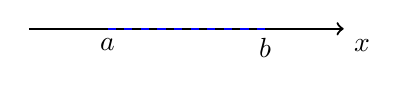
\begin{tikzpicture}
        \draw[->, thick] (-2, 0) -- (2, 0) node[anchor=north west] {$x$};

        \node[below] at (-1, 0) {$a$};
        \node[below] at (1, 0) {$b$};
        \draw[dashed, thick, color=blue] (-1, 0) -- (1, 0);
    \end{tikzpicture}
\end{center}

\subsection{Definition of Unisolvence}
Unisolvence is a property that ensures the existence of a unique nodal basis.
\begin{definition}{Unisolvence}{unisolvence}
    $\mathcal{N}$ determines $\mathcal{P}$ if for $\psi \in \mathcal{P}$ with $N(\psi) = 0$ for all $N \in \mathcal{N}$ implies $\psi = 0$.
\end{definition}

\subsection{Definition of a Hyperplane}
\begin{definition}{Hyperplane}{hyperplane}
    We call $\{x \, : \, L(x) = 0\}$ a hyperplane if $L$ is a non-degenerate.
\end{definition}

We abuse notation referring to $L$ as \emph{the hyperplane}.

\begin{lemma}{Deconstruction Lemma (DL)}{deconstruction-lemma}
    Let $P$ be a polynomial of degree $\deg(P) = d \geq 1$ vanishing on the hyperplane $L$. Then we have:
    \[
        P = L Q
    \]
    where $\deg(Q) = d - 1$.
\end{lemma}
\begin{proof}
    without loss of generality (w.l.o.g.) we may consider $L(x) = x_n$ (where $x \in \mathbb{R}^n$), i.e. the hyperplane is described by $L(\substack{\hat{x} \\ 0}) = 0$ where $x = [\hat{x}, x_n]$.
    We see that $P(\substack{\hat{x} \\ 0}) = 0$. Since $\deg(P) = d$ we can write:
    \[
        P(\substack{\hat{x} \\ x_n}) = \sum_{j=0}^d \sum_{|\hat{i}| \leq d - j} C_{\hat{i}j} \hat{x}^{\hat{i}} x_n^j \quad \begin{cases}
             & \hat{x} = (x_1, x_2, \ldots, x_{n-1}) \\
             & \hat{i} = (i_1, i_2, \ldots, i_{n-1})
        \end{cases}
    \]
    Letting $x_n = 0$ gives:
    \[
        P(\substack{\hat{x} \\ 0}) = \sum_{|\hat{i}| \leq d} C_{\hat{i}0} \hat{x}^{\hat{i}} = 0
    \]
    implying $C_{\hat{i}0} = 0$ for $|\hat{i}| \leq d$. This tells us that:
    \[
        P(\substack{\hat{x} \\ x_n}) = \sum_{j=1}^d \sum_{|\hat{i}| \leq d - j} C_{\hat{i}j} \hat{x}^{\hat{i}} x_n^j = x_n \underbrace{\sum_{j=1}^d \sum_{|\hat{i}| \leq d - j} C_{\hat{i}j} \hat{x}^{\hat{i}} x_n^{j-1}}_{Q(\substack{\hat{x} \\ x_n})} = x_n Q(\substack{\hat{x} \\ x_n}) = L(x) Q(x)
    \]
    where $\deg(Q) = d - 1$.\qed
\end{proof}

We begin focusing on \textbf{triangular elements:}

\subsection{Triangular elements}
Let $\mathcal{K}$ be any triangle and $\mathcal{P}_k$ be the set of polynomials (in two variables) of degree $\deg(P) \leq k$.

The most standard finite element is the \emph{linear ($k=1$) Lagrange element} defined by:

\begin{definition}{Linear Lagrange element}{linear-lagrange-element}
    Let $\mathcal{P} = P_1$ and $\mathcal{N} = \{N_1, N_2, N_3\}$ (as $\dim(P_1) = 3$) where:
    \[
        N_i(v) = v(z_i) \quad \text{ for vertices } z_1, z_2, z_3 \text{ of } \mathcal{K}
    \]
\end{definition}
\begin{center}
    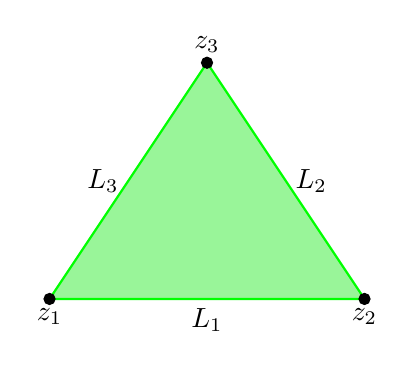
\begin{tikzpicture}
        \draw[thick, color=green, fill=green!90!black, fill opacity=0.4] (0, 0) -- (4, 0) -- (2, 3) -- cycle;
        \node[below] at (0, 0) {$z_1$};
        \node[below] at (4, 0) {$z_2$};
        \node[above] at (2, 3) {$z_3$};

        \filldraw[black] (0, 0) circle (2pt);
        \filldraw[black] (4, 0) circle (2pt);
        \filldraw[black] (2, 3) circle (2pt);

        % Include labels for edges L_i
        \node[below] at (2, 0) {$L_1$};
        \node[right] at (3, 1.5) {$L_2$};
        \node[left] at (1, 1.5) {$L_3$};
    \end{tikzpicture}
\end{center}
\begin{itemize}
    \item $\cdot$ represents nodes $z_i$.
    \item $L_i$ represents the edges.
\end{itemize}

Let's check this satisfies the definition of a finite element, to do this we need to show that $\mathcal{N}$ determines $\mathcal{P}_1$:
\begin{proof}[Proof that $\mathcal{N}=\{N_1, N_2, N_3\}$ determines $\mathcal{P}_1$]

    \medskip

    Let $L_1, L_2, L_3$ be linear functions describing the lines/edges of the triangle $\mathcal{K}$.
    \medskip
    Suppose we have a polynomial $P \in \mathcal{P}_1$ which vanishes on the nodes $z_1, z_2, z_3$.
    \medskip
    Since $P|_{L_1} = 0$ is linear in one variable and vanishes at two points, $P$ must vanish on the entire line $L_1$ s.t. $P|_{L_1} = 0$.
    By \emph{Deconstruction lemma \ref{lem:deconstruction-lemma}} we have $P = L_1 c$ where $c$ is a constant (since $\deg(P) = 1$).

    \[
        P(z_1) = c L_1(z_1) = 0 \implies c = 0 \quad \text{as} \quad L_1(z_1) \neq 0 \implies P = 0
    \]
    we have $P \equiv 0$ and can conclude that $\mathcal{N}$ determines $\mathcal{P}_1$ (and is a finite element).\qed
\end{proof}

This choice of element is not unique (but it is preferred).

Another valid element could be as follows:
\begin{center}
    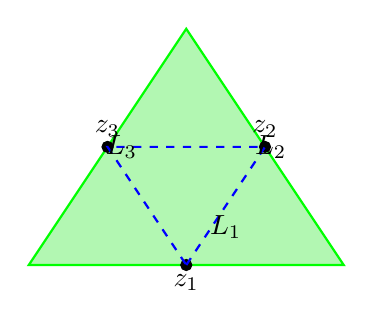
\begin{tikzpicture}
        \draw[thick, color=green, fill=green!90!black, fill opacity=0.3] (0, 0) -- (4, 0) -- (2, 3) -- cycle;
        \node[below] at (2, 0) {$z_1$};
        \node[above] at (3, 1.5) {$z_2$};
        \node[above] at (1, 1.5) {$z_3$};

        \filldraw[black] (2, 0) circle (2pt);
        \filldraw[black] (3, 1.5) circle (2pt);
        \filldraw[black] (1, 1.5) circle (2pt);

        % dashed lines between nodes
        \draw[dashed, thick, color=blue] (2, 0) -- (3, 1.5) -- (1, 1.5) -- cycle;

        % Include labels for edges L_i
        \node[below] at (2.5, 0.75) {$L_1$};
        \node[right] at (2.75, 1.5) {$L_2$};
        \node[left] at (1.5, 1.5) {$L_3$};
    \end{tikzpicture}
\end{center}

\begin{example}{$k=2$ triangular element}{}
    Let $\mathcal{P} = P_2$ and $\mathcal{N} = \{N_1, N_2, N_3, N_4, N_5, N_6\}$ (as $\dim(P_2) = 6$) where:
    \[
        N_i(v) =
        \begin{cases}
             & v(z_i), \quad i = 1, 2, 3 \text{ (vertices) }           \\
             & v(z_i), \quad i = 4, 5, 6 \text{ (midpoints of edges) }
        \end{cases}
    \]
    \begin{center}
        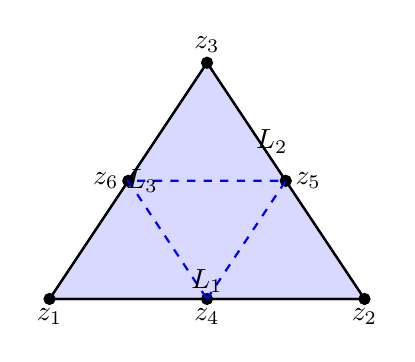
\begin{tikzpicture}
            \draw[thick, fill=blue!50, fill opacity=0.3] (0, 0) -- (4, 0) -- (2, 3) -- cycle;
            \draw[thick] (0, 0) -- (4, 0) -- (2, 3) -- cycle;
            \node[below] at (0, 0) {$z_1$};
            \node[below] at (4, 0) {$z_2$};
            \node[above] at (2, 3) {$z_3$};
            \node[below] at (2, 0) {$z_4$};
            \node[right] at (3, 1.5) {$z_5$};
            \node[left] at (1, 1.5) {$z_6$};

            \filldraw[black] (0, 0) circle (2pt);
            \filldraw[black] (4, 0) circle (2pt);
            \filldraw[black] (2, 3) circle (2pt);
            \filldraw[black] (2, 0) circle (2pt);
            \filldraw[black] (3, 1.5) circle (2pt);
            \filldraw[black] (1, 1.5) circle (2pt);


            % dashed lines between midpoints
            \draw[dashed, thick, color=blue] (2, 0) -- (3, 1.5) -- (1, 1.5) -- cycle;

            % Include labels for edges L_i
            \node[below] at (2, 0.5) {$L_1$};
            \node[right] at (2.5, 2) {$L_2$};
            \node[left] at (1.5, 1.5) {$L_3$};
        \end{tikzpicture}
    \end{center}
    To confirm this is a finite element we need to check that $\mathcal{N}$ determines $\mathcal{P}_2$:

    Suppose $P \in \mathcal{P}_2$ vanishes at all nodes $z_i$. Since $P|_{L_1}$ is quadratic in one variable and vanishes at $3$ points, $P|_{L_1} = 0$.

    By \emph{(DL)} we have $P = L_1 Q_1$ with $\deg(Q_1) = \deg(P) - 1 = 1$.
    As $P|_{L_2} = 0$ we have $L_1Q_1|_{L_2} = 0$. So $Q_1|_{L_2} = 0$ (a.e.) as $L_1(z_1) \neq 0$ except possible at $z_3$.
    By continuity of $Q_1$ we have $Q_1|_{L_2} = 0$.

    Applying \emph{(DL)} again we find $Q_1 = L_2 Q_2$ with $\deg(Q_2) = \deg(Q_1) - 1 = 0$.
    $\implies Q_2$ is a constant ($c$) and $P = c L_1 L_2$. Observe that $P(z_6) = 0$ and is not on $L_1$ or $L_2$, so $P(z_6) = c L_1(z_6) L_2(z_6) = 0 \implies c = 0$ as $L_1(z_6), L_2(z_6) \neq 0$.

    Thus $P \equiv 0$ and $\mathcal{N}$ determines $\mathcal{P}_2$, so it is a finite element.\qed

\end{example}

\section{Lecture 12: 25.09.2025}
\begin{example}{General Lagrange element}{}
    \[
        \mathcal{N}_k = \{N_i\}_{i=1}^{\frac12(k+1)(k+2)}, \quad
        N_i =
        \begin{cases}
            3 \text{ Vector Nodes}             \\
            3(k-1) \text{ Distinct Edge Nodes} \\
            \frac12(k-1)(k-2) \text{ Interior Nodes}
        \end{cases}
    \]
    With interior points chosen to determine $\mathbb{P}_k$.

    Let $k=3$ for the moment:

    \begin{center}
        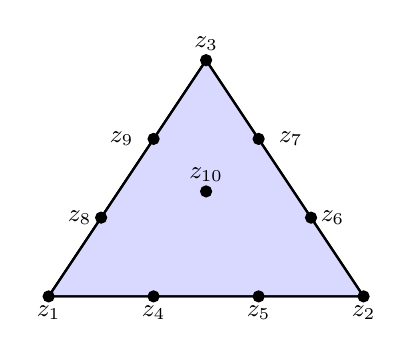
\begin{tikzpicture}[font=\small]
            \draw[thick, fill=blue!50, fill opacity=0.3] (0, 0) -- (4, 0) -- (2, 3) -- cycle;
            \draw[thick] (0, 0) -- (4, 0) -- (2, 3) -- cycle;
            \node[below] at (0, 0) {$z_1$};
            \node[below] at (4, 0) {$z_2$};
            \node[above] at (2, 3) {$z_3$};
            % Edge nodes for k=3: two per edge
            \node[below] at (1.333, 0) {$z_4$};
            \node[below] at (2.667, 0) {$z_5$};
            \node[right] at (3.333, 1) {$z_6$};
            \node[right] at (2.8, 2) {$z_7$};
            \node[left] at (0.667, 1) {$z_8$};
            \node[left] at (1.2, 2) {$z_9$};
            % Interior node
            \node[above] at (2, 1.333) {$z_{10}$};

            \filldraw[black] (0, 0) circle (2pt);
            \filldraw[black] (4, 0) circle (2pt);
            \filldraw[black] (2, 3) circle (2pt);
            \filldraw[black] (1.333, 0) circle (2pt);
            \filldraw[black] (2.667, 0) circle (2pt);
            \filldraw[black] (3.333, 1) circle (2pt);
            \filldraw[black] (2.667, 2) circle (2pt);
            \filldraw[black] (0.667, 1) circle (2pt);
            \filldraw[black] (1.333, 2) circle (2pt);
            \filldraw[black] (2, 1.333) circle (2pt);
        \end{tikzpicture}
    \end{center}

    For $k=4$:
    \begin{center}
        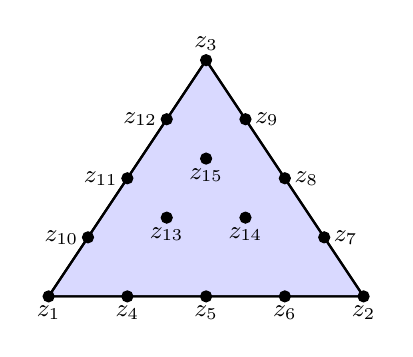
\begin{tikzpicture}[font=\small]
            \draw[thick, fill=blue!50, fill opacity=0.3] (0, 0) -- (4, 0) -- (2, 3) -- cycle;
            \draw[thick] (0, 0) -- (4, 0) -- (2, 3) -- cycle;
            \filldraw[black] (0, 0) circle (2pt) node[below] {$z_1$};
            \filldraw[black] (4, 0) circle (2pt) node[below] {$z_2$};
            \filldraw[black] (2, 3) circle (2pt) node[above] {$z_3$};
            % Edge nodes for k=4: three per edge
            \filldraw[black] (1, 0) circle (2pt) node[below] {$z_4$};
            \filldraw[black] (2, 0) circle (2pt) node[below] {$z_5$};
            \filldraw[black] (3, 0) circle (2pt) node[below] {$z_6$};
            \filldraw[black] (3.5, 0.75) circle (2pt) node[right] {$z_7$};
            \filldraw[black] (3, 1.5) circle (2pt) node[right] {$z_8$};
            \filldraw[black] (2.5, 2.25) circle (2pt) node[right] {$z_9$};
            \filldraw[black] (0.5, 0.75) circle (2pt) node[left] {$z_{10}$};
            \filldraw[black] (1, 1.5) circle (2pt) node[left] {$z_{11}$};
            \filldraw[black] (1.5, 2.25) circle (2pt) node[left] {$z_{12}$};

            % Interior nodes
            \filldraw[black] (1.5, 1) circle (2pt) node[below] {$z_{13}$};
            \filldraw[black] (2.5, 1) circle (2pt) node[below] {$z_{14}$};
            \filldraw[black] (2, 1.75) circle (2pt) node[below] {$z_{15}$};
        \end{tikzpicture}
    \end{center}
    The interior point makes a $\mathbb{P}_1$ element that is a triangle.\footnote{The proof is left as an exercise for the reader.}
\end{example}

\subsection{The Cubic Hermite}
Let $\mathcal{P} = \mathbb{P}_3$, where $\cdot$ be a point evaluation and $\odot$ a derivative evaluation, then the FE is given by $\mathcal{N} = \{N_1, \dots, N_10\}$

Abridged version to skip some technical details:

Showing this is an FE by assuming $p \in \mathbb{P}_3$ s.t.
\[
N_i(p) = 0 \quad \forall \, i
\]

Restricting to $L_1$ then:
\[
\begin{cases}
& p(z_2)= p'(z_2) = 0 \\
& p(z_3) = p'(z_3) = 0
\end{cases}
\]
where the derivative is along the edge.
\begin{center}
    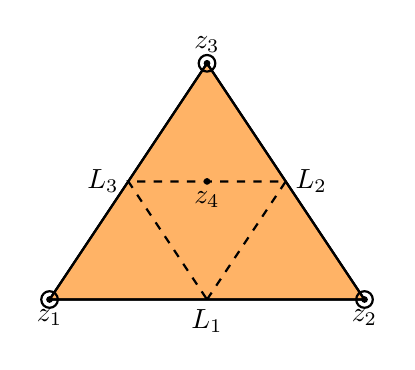
\begin{tikzpicture}
        \draw[thick, fill=orange, fill opacity=0.6] (0, 0) -- (4, 0) -- (2, 3) -- cycle;
        \draw[thick] (0, 0) -- (4, 0) -- (2, 3) -- cycle;
        \draw[thick, dashed] (2,0) -- (3, 1.5) -- (1,1.5) -- cycle;
        \draw[thick] (0, 0) circle (3pt) node[below] {$z_1$};
        \draw[thick] (4, 0) circle (3pt) node[below] {$z_2$};
        \draw[thick] (2, 3) circle (3pt) node[above] {$z_3$};
        \filldraw (2, 1.5) circle (1pt) node[below] {$z_4$};
        \filldraw (0, 0) circle (1pt);
        \filldraw (4, 0) circle (1pt);
        \filldraw (2, 3) circle (1pt);

        % Include labels for edges L_i
        \node[below] at (2, 0) {$L_1$};
        \node[right] at (3, 1.5) {$L_2$};
        \node[left] at (1, 1.5) {$L_3$};
    \end{tikzpicture}
\end{center}

The only cubic polynomial with 4 roots is $0$: $p\lvert_{L_1} \equiv 0$ and the same follows for $p\lvert_{L_2}$ and $p\lvert_{L_3}$.

By (DL) we have:

\[
\begin{aligned}
    p &= c L_1 L_2 L_3 &\\
    L_i(z_4) &\neq 0 & i = 1,2,3 \\
    p(z_4) &= 0 \implies c = 0 &\implies \boxed{p = 0}
\end{aligned}
\]
For a more complete proof one has to show in detail that $p = L_i Q_i$ and that if $p(x) = 0$ and $L_i \neq Q_i$ (a.e.).

\subsection{Defining the derivatives}
we need two points to derive the derivatives at a point.
In practice one might use directional derivatives.
Then the Hermite element can be drawn as follows (where the arrows is its derivative):

\begin{center}
    \begin{tikzpicture}
        \draw[thick, fill=blue!50, fill opacity=0.4] (0, 0) -- (4, 0) -- (2, 3) -- cycle;
        \filldraw[black] (0, 0) circle (2pt) node[below] at (0, 0) {$z_1$};
        \filldraw[black] (4, 0) circle (2pt) node[below] at (4, 0) {$z_2$};
        \filldraw[black] (2, 3) circle (2pt) node[above] at (2, 3) {$z_3$};
        \draw[->, thick, spaceblack] (0,0) -- (1,0);
        \draw[->, thick, spaceblack] (0,0) -- (0,1);
        \draw[->, thick, spaceblack] (4,0) -- (5,0);
        \draw[->, thick, spaceblack] (4,0) -- (4,1);
        \draw[->, thick, spaceblack] (2,3) -- (3,3);
        \draw[->, thick, spaceblack] (2,3) -- (2,4);


        % Include labels for edges L_i
        \node[below] at (2, 0) {$L_1$};
        \node[right] at (3, 1.5) {$L_2$};
        \node[left] at (1, 1.5) {$L_3$};
    \end{tikzpicture}
\end{center}
\textbf{In general} the Hermite elements have $\frac12(k+1)(k+2) \, DoF = \# \, Nodes$  where the nodal variables are:
\[
N_i =
\begin{cases}
    3 \text{ Vertices}\\
    6 \text{ Derivatives}\\
    3(k-3) \text{ Edges} \\
    \frac12(k-2)(k-1) \text{ Interior}
\end{cases}
\]

% The Hermite element is not usually preferedover Lagrange
% but are an alt choice
% Example quintic Argyris Let D Ps in two variables and consider the
% 21 dimP dof where are pointevaluation and are istand2ⁿᵈderivati
% are normal derivatives at midpoint mi
% The proof is left as an exercise for the reader
% Proof in BS book

% To build a FE space we piece the elements together
% Def local interpolent for a FE 39,8 ur let i i k
% be the basis of N abasis for D
% The local interpolant is
% I v Nilu di
% Note v must be well defined Ni
% Eksample Consider spanned by the basisfunctions
% 1010 11,01
% 4,1 11 I y The interpolant is
% 926.9
% 9,6cg I Irv N Vaio 1 1 N VG.DE
% Vlan I
% As before the interpolant is invariant under composition
% Ikt Iq
% some more definitions
% Def Subdevision of a domain or is a finite collection
% of dement domain Ki
% s.t.int
% Ki nint Kj if itj the empty domain
% and µ K I
% Def A triangelization is a subderision where no ventet of any
% triangle lies in the interior of an edge of another triangle
% vertecis can share information
% edges can not
% ok not ok
% as ventet
% toutches an
% edgeDef Interpolant Let or have some triangelazation T of KPN
% the FE fixingm to the highest orde derivative in the nodal
% variables we can define the interpolant of a function fee a
% It
% Eit KIET
% µ
% To build a conforming FES we need to enforce conditions between
% elements Enforcing C continuity we can obtain a FES VG ECMER
% elements Through enforcing continuity the Lagrange and
% Hamite elements are a subspace of C
% C elements Enforcing C continuity the Argyri's elements are
% a subspace of C
% Let's Focus on Lagrange elements
% Det Diameter Given a set 5 diamCs 11 911
% Def Mesh conditions Let a be given and Ta be a family of
% triangulations sit
% max diam T Te Tu h diamle for och El
% further define B sit for any ET the closed convex hull
% of UB is contained in T
% We must work within convex shapes
% The family of meshes is quasi uniform if 79 0 sit
% min dium B TE Ta ghdiamler COD
% The family is non degenerate if 75 SO s t
% TE Tu and 410,1
% diamLB 2g diam T